\documentclass[lualatex,ja=standard,a4paper,12pt]{bxjsarticle}
\usepackage{amsmath, amssymb, amsthm, bm}
\usepackage{geometry}
\usepackage{xcolor}
\usepackage{tcolorbox}
\usepackage{booktabs}
\usepackage{array}
\usepackage{tikz}

\geometry{margin=25mm}

\tcbuselibrary{theorems, skins, breakable}

\newtcolorbox{defbox}[1]{
  colback=blue!5, colframe=blue!60!black,
  fonttitle=\bfseries, title={#1}, arc=3pt, breakable
}
\newtcolorbox{thmbox}[1]{
  colback=green!5, colframe=green!50!black,
  fonttitle=\bfseries, title={#1}, arc=3pt, breakable
}
\newtcolorbox{pointbox}{
  colback=orange!8, colframe=orange!70!black,
  fonttitle=\bfseries, title={ポイント}, arc=3pt, breakable
}
\newtcolorbox{exbox}[1]{
  colback=gray!6, colframe=gray!50,
  fonttitle=\bfseries, title={例：#1}, arc=3pt, breakable
}
\newtcolorbox{derivbox}{
  colback=purple!4, colframe=purple!50!black,
  fonttitle=\bfseries, title={導出}, arc=3pt, breakable
}
\newtcolorbox{warningbox}{
  colback=red!5, colframe=red!60!black,
  fonttitle=\bfseries, title={注意}, arc=3pt, breakable
}

\newcommand{\mvn}{\mathrm{MVN}}

\title{補足資料 \\[6pt]
       \textbf{多変量正規分布（MVN）} \\[4pt]
       {\normalsize 第11章を読むための準備　ゼミ資料}}
\author{}
\date{}

\begin{document}
\maketitle
\thispagestyle{empty}

% ===========================
\section{なぜ必要か}
% ===========================

第11章の階層回帰モデルでは
\[
  \bm{\beta}_1, \ldots, \bm{\beta}_m \overset{\text{i.i.d.}}{\sim} \mvn(\bm{\theta}, \Sigma)
\]
という式が何度も出てくる．$\mvn$ は \textbf{Multivariate Normal distribution}（\textbf{多変量正規分布}）の略で，
普通の正規分布を\textbf{ベクトル}（いくつかの数の組）に拡張したものである（教科書第7章）．

\medskip
数学の点数の例では，学校 $j$ の回帰係数は2つの数の組
\[
  \bm{\beta}_j = \begin{pmatrix} \beta_{1,j} \\ \beta_{2,j} \end{pmatrix}
  = \begin{pmatrix} \text{切片（学校の平均点）} \\ \text{傾き（SES の効果）} \end{pmatrix}
\]
であり，「100校の（切片，傾き）の組がどうばらついているか」を表すのに $\mvn$ を使う．

% ===========================
\section{定義}
% ===========================

\begin{defbox}{多変量正規分布}
$p$ 次元の確率ベクトル $\bm{Y} = (Y_1, \ldots, Y_p)^\top$ の密度が
\[
  p(\bm{y} \mid \bm{\theta}, \Sigma)
  = (2\pi)^{-p/2}\,|\Sigma|^{-1/2}
    \exp\!\Bigl\{-\tfrac12(\bm{y} - \bm{\theta})^\top \Sigma^{-1}(\bm{y} - \bm{\theta})\Bigr\}
\]
で与えられるとき，$\bm{Y} \sim \mvn(\bm{\theta}, \Sigma)$ と書く．
\begin{itemize}
  \item $\bm{\theta} = E[\bm{Y}]$：\textbf{平均ベクトル}（$p$ 次元）
  \item $\Sigma = \mathrm{Cov}[\bm{Y}]$：\textbf{共分散行列}（$p \times p$，対称・正定値）
  \item $|\Sigma|$ は $\Sigma$ の行列式
\end{itemize}
\end{defbox}

\subsection{1次元の正規分布との対応}

\begin{center}
\renewcommand{\arraystretch}{1.6}
\begin{tabular}{lll}
\toprule
 & 正規分布 & 多変量正規分布 \\
\midrule
扱う量 & 数 $y$ & ベクトル $\bm{y}$ \\
中心 & 平均 $\theta$ & 平均ベクトル $\bm{\theta}$ \\
広がり & 分散 $\sigma^2$ & 共分散行列 $\Sigma$ \\
正規化定数 & $(2\pi\sigma^2)^{-1/2}$ & $(2\pi)^{-p/2}|\Sigma|^{-1/2}$ \\
指数の中 & $-\dfrac{(y-\theta)^2}{2\sigma^2}$ & $-\tfrac12(\bm{y}-\bm{\theta})^\top\Sigma^{-1}(\bm{y}-\bm{\theta})$ \\
\bottomrule
\end{tabular}
\end{center}

\noindent $p = 1$ とすると $\Sigma = \sigma^2$，$\Sigma^{-1} = 1/\sigma^2$，$|\Sigma| = \sigma^2$ なので，
普通の正規分布の密度にぴったり戻る．
「$1/\sigma^2$ で割る」が「$\Sigma^{-1}$ を両側から挟む」に置き換わったと思えばよい．

\subsection{共分散行列の中身}

$p = 2$ の場合，
\[
  \Sigma = \begin{pmatrix}
    \sigma_1^2 & \sigma_{12} \\
    \sigma_{12} & \sigma_2^2
  \end{pmatrix}
  = \begin{pmatrix}
    \mathrm{Var}[Y_1] & \mathrm{Cov}[Y_1, Y_2] \\
    \mathrm{Cov}[Y_1, Y_2] & \mathrm{Var}[Y_2]
  \end{pmatrix},
  \qquad
  \rho = \frac{\sigma_{12}}{\sigma_1\sigma_2}\;\text{（相関係数）}.
\]
\begin{itemize}
  \item \textbf{対角成分}：各成分のばらつき
  \item \textbf{非対角成分}：2つの成分が\textbf{一緒に動く傾向}（相関）
\end{itemize}

% ===========================
\section{形のイメージ}
% ===========================

2次元の $\mvn$ の密度は「山」の形をしていて，等高線は\textbf{楕円}になる．
下の図は $\bm{\theta} = (0, 0)$，$\sigma_1 = \sigma_2 = 1$ で相関 $\rho$ だけを変えたときの等高線である
（内側の楕円が $(\bm{y}-\bm{\theta})^\top\Sigma^{-1}(\bm{y}-\bm{\theta}) = 1$，外側が $= 4$）．

\begin{center}
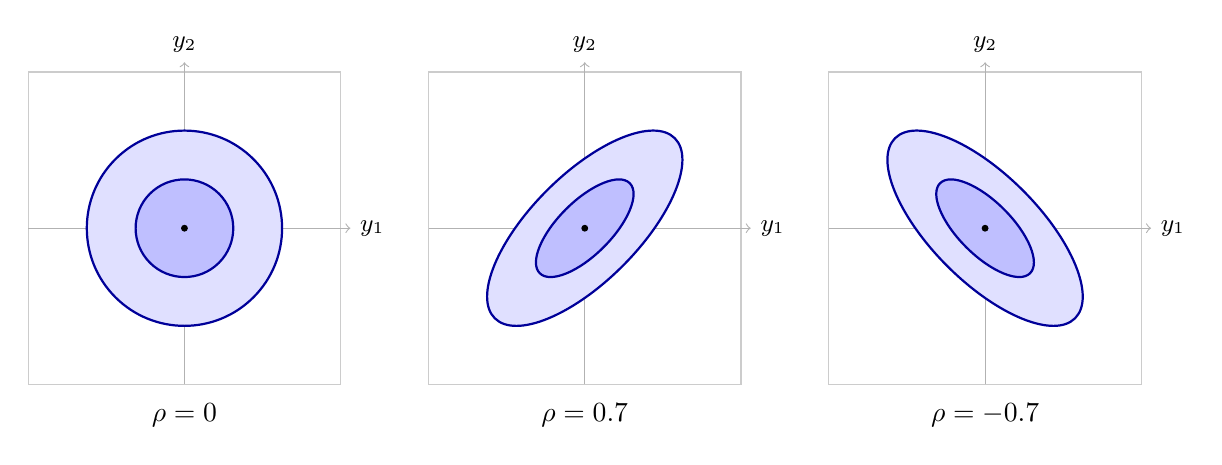
\begin{tikzpicture}[scale=0.62]
  \foreach \r/\x/\lab in {0/0/{$\rho = 0$}, 0.7/8.2/{$\rho = 0.7$}, -0.7/16.4/{$\rho = -0.7$}} {
    \begin{scope}[xshift=\x cm]
      \draw[gray!40] (-3.2,-3.2) rectangle (3.2,3.2);
      \draw[gray!60, ->] (-3.2,0) -- (3.4,0) node[right, black] {\small $y_1$};
      \draw[gray!60, ->] (0,-3.2) -- (0,3.4) node[above, black] {\small $y_2$};
      \pgfmathsetmacro{\a}{sqrt(1+\r)}
      \pgfmathsetmacro{\b}{sqrt(1-\r)}
      \fill[blue!12, rotate=45] (0,0) ellipse ({2*\a} and {2*\b});
      \draw[blue!60!black, thick, rotate=45] (0,0) ellipse ({2*\a} and {2*\b});
      \fill[blue!25, rotate=45] (0,0) ellipse ({\a} and {\b});
      \draw[blue!60!black, thick, rotate=45] (0,0) ellipse ({\a} and {\b});
      \fill (0,0) circle (2pt);
      \node[below] at (0,-3.4) {\lab};
    \end{scope}
  }
\end{tikzpicture}
\end{center}

\begin{itemize}
  \item $\rho = 0$：円．$y_1$ が大きくても $y_2$ について何もわからない．
  \item $\rho > 0$：右上がりの楕円．$y_1$ が大きいと $y_2$ も大きくなりやすい．
  \item $\rho < 0$：右下がりの楕円．$y_1$ が大きいと $y_2$ は小さくなりやすい．
\end{itemize}

\begin{exbox}{第11章の $\bm{\beta}_j \sim \mvn(\bm{\theta}, \Sigma)$}
100校の（切片 $\beta_{1,j}$，傾き $\beta_{2,j}$）を平面上の点として打つと，楕円形の雲になる，というモデル．
\begin{itemize}
  \item $\bm{\theta} = (\theta_1, \theta_2)$：雲の中心＝学校全体の平均的な切片と傾き
  \item $\Sigma_{11}, \Sigma_{22}$：切片のばらつき，傾きのばらつき
  \item $\Sigma_{12}$：「平均点が高い学校ほど SES の効果が大きい（小さい）」といった\textbf{切片と傾きの関係}
\end{itemize}
切片と傾きに別々の1次元正規分布を当てると，$\Sigma_{12}$ にあたる関係が表せない．
だから $\mvn$ を使い，$\Sigma$ ごと推定する．
\end{exbox}

% ===========================
\section{よく使う性質}
% ===========================

\begin{thmbox}{性質1：線形変換しても MVN}
$\bm{Y} \sim \mvn(\bm{\theta}, \Sigma)$，$A$ を定数行列，$\bm{c}$ を定数ベクトルとすると
\[
  A\bm{Y} + \bm{c} \sim \mvn(A\bm{\theta} + \bm{c},\; A\Sigma A^\top).
\]
\end{thmbox}

\noindent 平均は $E[A\bm{Y} + \bm{c}] = A\bm{\theta} + \bm{c}$，
共分散は $\mathrm{Cov}[A\bm{Y}] = E[A(\bm{Y}-\bm{\theta})(\bm{Y}-\bm{\theta})^\top A^\top] = A\Sigma A^\top$．
1次元の「$aY + c$ の分散は $a^2\sigma^2$」の行列版である．

\begin{thmbox}{性質2：独立な MVN の和も MVN}
$\bm{U} \sim \mvn(\bm{a}, \Sigma_U)$ と $\bm{V} \sim \mvn(\bm{b}, \Sigma_V)$ が独立なら
\[
  \bm{U} + \bm{V} \sim \mvn(\bm{a} + \bm{b},\; \Sigma_U + \Sigma_V).
\]
\end{thmbox}

\begin{exbox}{第11章：同じ学校の生徒はなぜ相関するか}
$\bm{\beta}_j = \bm{\theta} + \bm{\gamma}_j$，$\bm{\gamma}_j \sim \mvn(\bm{0}, \Sigma)$ とすると
\[
  \bm{Y}_j = X_j\bm{\theta} + \underbrace{X_j\bm{\gamma}_j}_{\text{性質1：}\mvn(\bm{0},\, X_j\Sigma X_j^\top)}
  + \underbrace{\bm{\epsilon}_j}_{\mvn(\bm{0},\, \sigma^2 I)}.
\]
2つは独立なので性質2より
\[
  \bm{Y}_j \sim \mvn\bigl(X_j\bm{\theta},\; X_j\Sigma X_j^\top + \sigma^2 I\bigr).
\]
$\sigma^2 I$ は対角行列（生徒どうし独立）だが，$X_j\Sigma X_j^\top$ が非対角成分を持つので，
$\bm{\beta}_j$ を知らない状態では\textbf{同じ学校の生徒の点数は相関する}．
\end{exbox}

\begin{thmbox}{性質3：MVN では「無相関 $\Leftrightarrow$ 独立」}
$\bm{Y} \sim \mvn$ で，$\Sigma$ が対角行列（すべての共分散が0）なら，各成分 $Y_1, \ldots, Y_p$ は\textbf{独立}．
\end{thmbox}

\noindent 対角なら $\Sigma^{-1}$ も対角で，指数の中が $-\sum_k (y_k - \theta_k)^2/(2\sigma_k^2)$ と成分ごとの和に分かれ，
密度が1次元正規密度の積になるからである．

\begin{warningbox}
一般の分布では「無相関でも独立とは限らない」．これは MVN の特別な性質である．
例えば $\bm{Y}_j \sim \mvn(X_j\bm{\beta}_j, \sigma^2 I)$ は
「$\bm{\beta}_j$ を条件にすれば学校 $j$ の生徒の点数は互いに独立」という意味になる．
\end{warningbox}

\begin{thmbox}{性質4：周辺分布も正規分布}
$\bm{Y} \sim \mvn(\bm{\theta}, \Sigma)$ の各成分は $Y_k \sim \mathrm{Normal}(\theta_k, \Sigma_{kk})$．
\end{thmbox}

\noindent 性質1で $A = (0, \ldots, 0, 1, 0, \ldots, 0)$（$k$ 番目だけ1）とすればよい．
第11章で「傾き $\tilde{\beta}_2$ の事後予測分布」を考えるときは，$\mvn(\bm{\theta}, \Sigma)$ から
$\tilde{\bm{\beta}}$ を引いて第2成分だけを見ている．

% ===========================
\section{事後分布で MVN を見抜く方法（平方完成）}
% ===========================

第11章の $\bm{\beta}_j$ や $\bm{\theta}$ の完全条件付き分布は，すべてこの方法で求めている．

\begin{thmbox}{MVN の核}
ベクトル $\bm{\beta}$ の密度が
\[
  p(\bm{\beta}) \propto \exp\Bigl\{-\tfrac12\bm{\beta}^\top A\bm{\beta} + \bm{\beta}^\top\bm{b}\Bigr\}
  \qquad\text{（$A$ は対称・正定値）}
\]
の形なら，$\bm{\beta} \sim \mvn(A^{-1}\bm{b},\; A^{-1})$．
\end{thmbox}

\begin{derivbox}
$\mvn(\bm{m}, V)$ の指数の中を展開すると
\[
  -\tfrac12(\bm{\beta} - \bm{m})^\top V^{-1}(\bm{\beta} - \bm{m})
  = -\tfrac12\bm{\beta}^\top V^{-1}\bm{\beta} + \bm{\beta}^\top V^{-1}\bm{m} \;-\; \tfrac12\bm{m}^\top V^{-1}\bm{m}.
\]
最後の項は $\bm{\beta}$ を含まない定数なので，比例の範囲では無視できる．
係数を見比べると $V^{-1} = A$，$V^{-1}\bm{m} = \bm{b}$，つまり $V = A^{-1}$，$\bm{m} = A^{-1}\bm{b}$．
1次元の「$\exp\{-\frac{a}{2}x^2 + bx\}$ なら $\mathrm{Normal}(b/a,\, 1/a)$」と全く同じ発想である．
\end{derivbox}

\begin{pointbox}
\textbf{使い方：}
\begin{enumerate}
  \item 事後分布のうち $\bm{\beta}$ を含む因子だけを集める（尤度 × 事前分布）．
  \item 指数の中を展開し，\textbf{$\bm{\beta}$ の2次の項}の係数行列を $A$，\textbf{1次の項}の係数ベクトルを $\bm{b}$ として読み取る．
  \item $\mvn(A^{-1}\bm{b},\, A^{-1})$ と答える．
\end{enumerate}
$A$ は「精度行列」（分散の逆）で，\textbf{精度は足し算}になる：事後の精度 ＝ 事前の精度 ＋ データの精度．
\end{pointbox}

\begin{exbox}{第11章の $\bm{\beta}_j$ の完全条件付き分布}
$\bm{\beta}_j$ を含む因子は
\[
  \exp\Bigl\{-\tfrac{1}{2\sigma^2}\|\bm{y}_j - X_j\bm{\beta}_j\|^2\Bigr\}
  \times \exp\Bigl\{-\tfrac12(\bm{\beta}_j - \bm{\theta})^\top\Sigma^{-1}(\bm{\beta}_j - \bm{\theta})\Bigr\}.
\]
展開して2次と1次の項を集めると
\[
  A = \underbrace{\Sigma^{-1}}_{\text{事前（グループ間）の精度}} + \underbrace{X_j^\top X_j/\sigma^2}_{\text{データの精度}},
  \qquad
  \bm{b} = \Sigma^{-1}\bm{\theta} + X_j^\top\bm{y}_j/\sigma^2.
\]
よって $\bm{\beta}_j \mid \cdots \sim \mvn(A^{-1}\bm{b},\, A^{-1})$．これが第11章の
$V_j = (\Sigma^{-1} + X_j^\top X_j/\sigma^2)^{-1}$，$\bm{m}_j = V_j(\Sigma^{-1}\bm{\theta} + X_j^\top\bm{y}_j/\sigma^2)$ である．
\end{exbox}

% ===========================
\section{共分散行列 $\Sigma$ の事前分布：逆ウィシャート分布}
% ===========================

第11章では $\Sigma$ も推定するので，$\Sigma$ にも事前分布が必要になる．
「行列の分布」として使うのが\textbf{逆ウィシャート分布}（inverse-Wishart）である（教科書7.3節）．

\begin{center}
\renewcommand{\arraystretch}{1.5}
\begin{tabular}{lll}
\toprule
 & 1次元の正規モデル & 多変量正規モデル \\
\midrule
推定する広がり & 分散 $\sigma^2$ & 共分散行列 $\Sigma$ \\
共役な事前分布 & 逆ガンマ分布 & 逆ウィシャート分布 \\
事後での更新 & 平方和 $\sum(y_i - \theta)^2$ を足す & 平方和行列 $\sum(\bm{y}_i - \bm{\theta})(\bm{y}_i - \bm{\theta})^\top$ を足す \\
\bottomrule
\end{tabular}
\end{center}

\begin{defbox}{逆ウィシャート分布（必要なところだけ）}
$\Sigma \sim \mathrm{inverse\text{-}Wishart}(\eta_0, S_0^{-1})$ のとき
\[
  E[\Sigma] = \frac{1}{\eta_0 - p - 1}\,S_0.
\]
$\eta_0$ は「事前のサンプル数」，$S_0$ は「事前の平方和行列」のように働く．
\end{defbox}

\noindent 第11章で $\eta_0 = p + 2$ とするのは，$E[\Sigma] = S_0$ になり，しかも自由度が最小限で事前分布が拡散的になるからである．
事後では $\eta_0 \to \eta_0 + m$，$S_0 \to S_0 + S_\theta$ と，「サンプル数」と「平方和行列」を足すだけで更新される．

% ===========================
\section{まとめ}
% ===========================

\begin{thmbox}{多変量正規分布のまとめ}
\begin{enumerate}
  \item $\mvn(\bm{\theta}, \Sigma)$ は正規分布のベクトル版．$\bm{\theta}$ が中心，$\Sigma$ が広がりと\textbf{成分間の相関}を表す．
  \item 2次元では密度の等高線が楕円になり，相関 $\rho$ の符号で楕円の傾きが決まる．
  \item 線形変換・独立な和・周辺分布をとっても MVN のまま．MVN では無相関なら独立．
  \item $\exp\{-\frac12\bm{\beta}^\top A\bm{\beta} + \bm{\beta}^\top\bm{b}\}$ の形なら $\mvn(A^{-1}\bm{b}, A^{-1})$．
        第11章の完全条件付き分布はすべてこれで求まる．
  \item 第11章の $\bm{\beta}_j \sim \mvn(\bm{\theta}, \Sigma)$ は，学校ごとの（切片，傾き）の組が楕円形の雲のようにばらつくというモデル．
        $\Sigma$ は逆ウィシャート分布で推定する．
\end{enumerate}
\end{thmbox}

\end{document}
